\documentclass[]{article}
\usepackage{lmodern}
\usepackage{amssymb,amsmath}
\usepackage{ifxetex,ifluatex}
\usepackage{fixltx2e} % provides \textsubscript
\ifnum 0\ifxetex 1\fi\ifluatex 1\fi=0 % if pdftex
  \usepackage[T1]{fontenc}
  \usepackage[utf8]{inputenc}
\else % if luatex or xelatex
  \ifxetex
    \usepackage{mathspec}
  \else
    \usepackage{fontspec}
  \fi
  \defaultfontfeatures{Ligatures=TeX,Scale=MatchLowercase}
  \newcommand{\euro}{€}
\fi
% use upquote if available, for straight quotes in verbatim environments
\IfFileExists{upquote.sty}{\usepackage{upquote}}{}
% use microtype if available
\IfFileExists{microtype.sty}{%
\usepackage{microtype}
\UseMicrotypeSet[protrusion]{basicmath} % disable protrusion for tt fonts
}{}
\usepackage[margin=1in]{geometry}
\usepackage{hyperref}
\PassOptionsToPackage{usenames,dvipsnames}{color} % color is loaded by hyperref
\hypersetup{unicode=true,
            pdftitle={Phoenix Tracker},
            pdfborder={0 0 0},
            breaklinks=true}
\urlstyle{same}  % don't use monospace font for urls
\usepackage{color}
\usepackage{fancyvrb}
\newcommand{\VerbBar}{|}
\newcommand{\VERB}{\Verb[commandchars=\\\{\}]}
\DefineVerbatimEnvironment{Highlighting}{Verbatim}{commandchars=\\\{\}}
% Add ',fontsize=\small' for more characters per line
\usepackage{framed}
\definecolor{shadecolor}{RGB}{248,248,248}
\newenvironment{Shaded}{\begin{snugshade}}{\end{snugshade}}
\newcommand{\KeywordTok}[1]{\textcolor[rgb]{0.13,0.29,0.53}{\textbf{{#1}}}}
\newcommand{\DataTypeTok}[1]{\textcolor[rgb]{0.13,0.29,0.53}{{#1}}}
\newcommand{\DecValTok}[1]{\textcolor[rgb]{0.00,0.00,0.81}{{#1}}}
\newcommand{\BaseNTok}[1]{\textcolor[rgb]{0.00,0.00,0.81}{{#1}}}
\newcommand{\FloatTok}[1]{\textcolor[rgb]{0.00,0.00,0.81}{{#1}}}
\newcommand{\ConstantTok}[1]{\textcolor[rgb]{0.00,0.00,0.00}{{#1}}}
\newcommand{\CharTok}[1]{\textcolor[rgb]{0.31,0.60,0.02}{{#1}}}
\newcommand{\SpecialCharTok}[1]{\textcolor[rgb]{0.00,0.00,0.00}{{#1}}}
\newcommand{\StringTok}[1]{\textcolor[rgb]{0.31,0.60,0.02}{{#1}}}
\newcommand{\VerbatimStringTok}[1]{\textcolor[rgb]{0.31,0.60,0.02}{{#1}}}
\newcommand{\SpecialStringTok}[1]{\textcolor[rgb]{0.31,0.60,0.02}{{#1}}}
\newcommand{\ImportTok}[1]{{#1}}
\newcommand{\CommentTok}[1]{\textcolor[rgb]{0.56,0.35,0.01}{\textit{{#1}}}}
\newcommand{\DocumentationTok}[1]{\textcolor[rgb]{0.56,0.35,0.01}{\textbf{\textit{{#1}}}}}
\newcommand{\AnnotationTok}[1]{\textcolor[rgb]{0.56,0.35,0.01}{\textbf{\textit{{#1}}}}}
\newcommand{\CommentVarTok}[1]{\textcolor[rgb]{0.56,0.35,0.01}{\textbf{\textit{{#1}}}}}
\newcommand{\OtherTok}[1]{\textcolor[rgb]{0.56,0.35,0.01}{{#1}}}
\newcommand{\FunctionTok}[1]{\textcolor[rgb]{0.00,0.00,0.00}{{#1}}}
\newcommand{\VariableTok}[1]{\textcolor[rgb]{0.00,0.00,0.00}{{#1}}}
\newcommand{\ControlFlowTok}[1]{\textcolor[rgb]{0.13,0.29,0.53}{\textbf{{#1}}}}
\newcommand{\OperatorTok}[1]{\textcolor[rgb]{0.81,0.36,0.00}{\textbf{{#1}}}}
\newcommand{\BuiltInTok}[1]{{#1}}
\newcommand{\ExtensionTok}[1]{{#1}}
\newcommand{\PreprocessorTok}[1]{\textcolor[rgb]{0.56,0.35,0.01}{\textit{{#1}}}}
\newcommand{\AttributeTok}[1]{\textcolor[rgb]{0.77,0.63,0.00}{{#1}}}
\newcommand{\RegionMarkerTok}[1]{{#1}}
\newcommand{\InformationTok}[1]{\textcolor[rgb]{0.56,0.35,0.01}{\textbf{\textit{{#1}}}}}
\newcommand{\WarningTok}[1]{\textcolor[rgb]{0.56,0.35,0.01}{\textbf{\textit{{#1}}}}}
\newcommand{\AlertTok}[1]{\textcolor[rgb]{0.94,0.16,0.16}{{#1}}}
\newcommand{\ErrorTok}[1]{\textcolor[rgb]{0.64,0.00,0.00}{\textbf{{#1}}}}
\newcommand{\NormalTok}[1]{{#1}}
\usepackage{longtable,booktabs}
\usepackage{graphicx,grffile}
\makeatletter
\def\maxwidth{\ifdim\Gin@nat@width>\linewidth\linewidth\else\Gin@nat@width\fi}
\def\maxheight{\ifdim\Gin@nat@height>\textheight\textheight\else\Gin@nat@height\fi}
\makeatother
% Scale images if necessary, so that they will not overflow the page
% margins by default, and it is still possible to overwrite the defaults
% using explicit options in \includegraphics[width, height, ...]{}
\setkeys{Gin}{width=\maxwidth,height=\maxheight,keepaspectratio}
\setlength{\parindent}{0pt}
\setlength{\parskip}{6pt plus 2pt minus 1pt}
\setlength{\emergencystretch}{3em}  % prevent overfull lines
\providecommand{\tightlist}{%
  \setlength{\itemsep}{0pt}\setlength{\parskip}{0pt}}
\setcounter{secnumdepth}{5}

%%% Use protect on footnotes to avoid problems with footnotes in titles
\let\rmarkdownfootnote\footnote%
\def\footnote{\protect\rmarkdownfootnote}

%%% Change title format to be more compact
\usepackage{titling}

% Create subtitle command for use in maketitle
\newcommand{\subtitle}[1]{
  \posttitle{
    \begin{center}\large#1\end{center}
    }
}

\setlength{\droptitle}{-2em}
  \title{Phoenix Tracker}
  \pretitle{\vspace{\droptitle}\centering\huge}
  \posttitle{\par}
  \author{}
  \preauthor{}\postauthor{}
  \date{}
  \predate{}\postdate{}


% Redefines (sub)paragraphs to behave more like sections
\ifx\paragraph\undefined\else
\let\oldparagraph\paragraph
\renewcommand{\paragraph}[1]{\oldparagraph{#1}\mbox{}}
\fi
\ifx\subparagraph\undefined\else
\let\oldsubparagraph\subparagraph
\renewcommand{\subparagraph}[1]{\oldsubparagraph{#1}\mbox{}}
\fi


\begin{document}
\maketitle

{
\setcounter{tocdepth}{2}
\tableofcontents
}
\section{Introduction}\label{introduction}

This project analyzes event data from the
\href{http://phoenixdata.org}{Phoenix Data Project}

\subsection{Getting Started}\label{getting-started}

Load the necessary packages.

\begin{Shaded}
\begin{Highlighting}[]
\KeywordTok{library}\NormalTok{(yaml)}
\KeywordTok{library}\NormalTok{(tidyverse)}
\end{Highlighting}
\end{Shaded}

\subsection{Loading Phoenix Dataset}\label{loading-phoenix-dataset}

The \texttt{phoenix.R} script provides a function that simplifies
downloading and loading the dataset. We set the start date to the
beginning of the year and load the dataset. The \texttt{phoenix\_load()}
function downloads the dataset if necessary.

\begin{Shaded}
\begin{Highlighting}[]
\KeywordTok{source}\NormalTok{(}\StringTok{'R/phoenix.R'}\NormalTok{)}

\NormalTok{config <-}\StringTok{ }\KeywordTok{yaml.load_file}\NormalTok{(}\StringTok{"config.yml"}\NormalTok{)}

\NormalTok{events <-}\StringTok{ }\KeywordTok{phoenix_load}\NormalTok{(config, }\DataTypeTok{start_date =} \StringTok{"2017-01-01"}\NormalTok{)}
\end{Highlighting}
\end{Shaded}

Let's see what's in the dataset

\begin{Shaded}
\begin{Highlighting}[]
\KeywordTok{str}\NormalTok{(events)}
\end{Highlighting}
\end{Shaded}

\begin{verbatim}
## 'data.frame':    104356 obs. of  26 variables:
##  $ EventID             : chr  "2867898_v1.3.0" "2867899_v1.3.0" "2867900_v1.3.0" "2867901_v1.3.0" ...
##  $ Date                : Date, format: "2017-01-02" "2016-12-23" ...
##  $ Year                : int  2017 2016 2016 2017 2017 2017 2017 2017 2017 2017 ...
##  $ Month               : int  1 12 12 1 1 1 1 1 1 1 ...
##  $ Day                 : int  2 23 29 2 2 2 2 1 1 2 ...
##  $ SourceActorFull     : chr  "COG" "MNCCHE" "IRN" "DEU" ...
##  $ SourceActorEntity   : chr  "COG" "MNC" "IRN" "DEU" ...
##  $ SourceActorRole     : chr  "" "" "" "" ...
##  $ SourceActorAttribute: chr  "" "CHE" "" "" ...
##  $ TargetActorFull     : chr  "MED" "USAGOV" "SYR" "GBR" ...
##  $ TargetActorEntity   : chr  "" "USA" "SYR" "GBR" ...
##  $ TargetActorRole     : chr  "" "GOV" "" "" ...
##  $ TargetActorAttribute: chr  "" "" "" "" ...
##  $ EventCode           : chr  "010" "010" "010" "042" ...
##  $ EventRootCode       : chr  "01" "01" "01" "04" ...
##  $ PentaClass          : chr  "0" "0" "0" "1" ...
##  $ GoldsteinScore      : num  0 0 0 1.9 -4.4 1.9 0 1 1.9 0 ...
##  $ Issues              : chr  "" "" "" "" ...
##  $ Lat                 : num  NA 39.8 55.8 51.5 39.9 ...
##  $ Lon                 : num  NA -98.5 37.616 -0.126 116.397 ...
##  $ LocationName        : chr  "" "United States" "Moscow" "London" ...
##  $ StateName           : chr  "" "" "Moskva" "England" ...
##  $ CountryCode         : chr  "" "USA" "RUS" "GBR" ...
##  $ SentenceID          : chr  "586a9d7beaae1f0001eec49c_1" "5869ac06dc0402000134e7ef_0" "5869ac72d57de600015a7951_1" "586a3e29172dca00014c31b9_2;586a2f7fe580470001f1b3d6_2;586a36dfc6faa00001190301_3" ...
##  $ URLs                : chr  "http://www.nation.co.ke/news/africa/DR-Congo-set-for-talks-on-implementing-crisis-deal/1066-3504894-k0ud9b/index.html" "http://www.thelocal.ch/20161223/swiss-bank-to-pay-billions-to-settle-securities-disputes" "http://www.jpost.com/Middle-East/Syrian-army-says-countrywide-ceasefire-to-start-midnight-Thursday-476890" "https://in.news.yahoo.com/china-launches-first-freight-train-london-113004033.html;http://www.shanghaidaily.com/nation/China-la"| __truncated__ ...
##  $ NewsSources         : chr  "kenya_nation" "local_switzerland" "jpost_me" "yahoo_india;shanghai_national;india_mint_econpol" ...
\end{verbatim}

Show selected columns

\begin{Shaded}
\begin{Highlighting}[]
\NormalTok{events %>%}
\StringTok{  }\KeywordTok{select}\NormalTok{(Date, SourceActorFull, TargetActorFull, EventCode, LocationName) %>%}
\StringTok{  }\KeywordTok{head}\NormalTok{()}
\end{Highlighting}
\end{Shaded}

\begin{verbatim}
##         Date SourceActorFull TargetActorFull EventCode  LocationName
## 1 2017-01-02             COG             MED       010              
## 2 2016-12-23          MNCCHE          USAGOV       010 United States
## 3 2016-12-29             IRN             SYR       010        Moscow
## 4 2017-01-02             DEU             GBR       042        London
## 5 2017-01-02             CHN             HKG       130       Beijing
## 6 2017-01-02       USAELIGOV          USAGOV       042
\end{verbatim}

\begin{center}\rule{0.5\linewidth}{\linethickness}\end{center}

\emph{Last Updated: Feb 06, 2017 1:13 AM}

\section{Activity}\label{activity}

\begin{Shaded}
\begin{Highlighting}[]
\KeywordTok{library}\NormalTok{(cshapes)}
\KeywordTok{library}\NormalTok{(countrycode)}
\KeywordTok{library}\NormalTok{(tidyverse)}
\KeywordTok{library}\NormalTok{(lubridate)}
\KeywordTok{library}\NormalTok{(broom)}
\KeywordTok{library}\NormalTok{(yaml)}
\KeywordTok{library}\NormalTok{(ggrepel)}
\end{Highlighting}
\end{Shaded}

\subsection{Loading Dataset}\label{loading-dataset}

Load Phoenix events and few other things we need for plotting.

\begin{Shaded}
\begin{Highlighting}[]
\KeywordTok{source}\NormalTok{(}\StringTok{'R/phoenix.R'}\NormalTok{)}

\NormalTok{config <-}\StringTok{ }\KeywordTok{yaml.load_file}\NormalTok{(}\StringTok{"config.yml"}\NormalTok{)}

\NormalTok{events <-}\StringTok{ }\KeywordTok{phoenix_load}\NormalTok{(config, }\StringTok{"2017-01-01"}\NormalTok{)}

\NormalTok{country_centroids <-}\StringTok{ }\KeywordTok{read_csv}\NormalTok{(config$google$centroids)}

\NormalTok{world_map <-}\StringTok{ }\KeywordTok{tidy}\NormalTok{(}\KeywordTok{cshp}\NormalTok{(}\KeywordTok{as.Date}\NormalTok{(}\StringTok{"2016-06-30"}\NormalTok{)), }\DataTypeTok{region =} \StringTok{"COWCODE"}\NormalTok{)}
\end{Highlighting}
\end{Shaded}

Function for summarizing events. Return value contains a list of nodes
and edges reprensenting dyadic events.

\begin{Shaded}
\begin{Highlighting}[]
\NormalTok{get_event_summary <-}\StringTok{ }\NormalTok{function(events, centroids, }\DataTypeTok{period =} \DecValTok{0}\NormalTok{) \{}
  \NormalTok{events <-}\StringTok{ }\NormalTok{events %>%}
\StringTok{    }\KeywordTok{filter}\NormalTok{(Date >=}\StringTok{ }\NormalTok{(}\KeywordTok{max}\NormalTok{(Date) -}\StringTok{ }\KeywordTok{days}\NormalTok{(period))) %>%}
\StringTok{    }\KeywordTok{filter}\NormalTok{(SourceActorRole ==}\StringTok{ "GOV"} \NormalTok{&}\StringTok{ }\NormalTok{TargetActorRole ==}\StringTok{ "GOV"}\NormalTok{)}
  
  \NormalTok{nodes <-}\StringTok{ }\NormalTok{events %>%}
\StringTok{    }\NormalTok{dplyr::}\KeywordTok{mutate}\NormalTok{(}\DataTypeTok{TargetActorEntity =} \KeywordTok{ifelse}\NormalTok{(SourceActorEntity ==}\StringTok{ }\NormalTok{TargetActorEntity, }\OtherTok{NA}\NormalTok{, TargetActorEntity)) %>%}
\StringTok{    }\KeywordTok{gather}\NormalTok{(ActorType, ActorEntity, SourceActorEntity, TargetActorEntity) %>%}
\StringTok{    }\KeywordTok{filter}\NormalTok{(!}\KeywordTok{is.na}\NormalTok{(ActorEntity), !(ActorEntity ==}\StringTok{ ""}\NormalTok{)) %>%}
\StringTok{    }\KeywordTok{group_by}\NormalTok{(ActorEntity) %>%}
\StringTok{    }\NormalTok{dplyr::}\KeywordTok{summarize}\NormalTok{(}\DataTypeTok{EventCount =} \KeywordTok{n}\NormalTok{()) %>%}
\StringTok{    }\NormalTok{dplyr::}\KeywordTok{mutate}\NormalTok{(}\DataTypeTok{CountryCode =} \KeywordTok{countrycode}\NormalTok{(ActorEntity, }\StringTok{"iso3c"}\NormalTok{, }\StringTok{"cown"}\NormalTok{), EventCount) %>%}
\StringTok{    }\KeywordTok{select}\NormalTok{(CountryCode, }\DataTypeTok{Country =} \NormalTok{ActorEntity, EventCount) %>%}
\StringTok{    }\KeywordTok{left_join}\NormalTok{(centroids, }\DataTypeTok{by =} \StringTok{"Country"}\NormalTok{) %>%}
\StringTok{    }\KeywordTok{arrange}\NormalTok{(}\KeywordTok{desc}\NormalTok{(EventCount)) }
  
  \NormalTok{edges <-}\StringTok{ }\NormalTok{events %>%}
\StringTok{    }\KeywordTok{filter}\NormalTok{(!}\KeywordTok{is.na}\NormalTok{(SourceActorEntity), !(SourceActorEntity ==}\StringTok{ ""}\NormalTok{),}
           \NormalTok{!}\KeywordTok{is.na}\NormalTok{(TargetActorEntity), !(TargetActorEntity ==}\StringTok{ ""}\NormalTok{),}
           \NormalTok{SourceActorEntity !=}\StringTok{ }\NormalTok{TargetActorEntity) %>%}
\StringTok{    }\KeywordTok{rowwise}\NormalTok{() %>%}
\StringTok{    }\NormalTok{dplyr::}\KeywordTok{mutate}\NormalTok{(}\DataTypeTok{Dyad =} \KeywordTok{paste}\NormalTok{(}\KeywordTok{sort}\NormalTok{(}\KeywordTok{c}\NormalTok{(SourceActorEntity, TargetActorEntity)), }\DataTypeTok{collapse =} \StringTok{"-"}\NormalTok{)) %>%}
\StringTok{    }\KeywordTok{ungroup}\NormalTok{() %>%}
\StringTok{    }\KeywordTok{group_by}\NormalTok{(Dyad) %>%}
\StringTok{    }\NormalTok{dplyr::}\KeywordTok{summarize}\NormalTok{(}\DataTypeTok{EventCount =} \KeywordTok{n}\NormalTok{()) %>%}
\StringTok{    }\KeywordTok{ungroup}\NormalTok{() %>%}
\StringTok{    }\KeywordTok{separate}\NormalTok{(Dyad, }\KeywordTok{c}\NormalTok{(}\StringTok{"SideA"}\NormalTok{, }\StringTok{"SideB"}\NormalTok{), }\StringTok{"-"}\NormalTok{, }\DataTypeTok{remove =} \OtherTok{FALSE}\NormalTok{) %>%}
\StringTok{    }\NormalTok{dplyr::}\KeywordTok{mutate}\NormalTok{(}\DataTypeTok{CountryA =} \KeywordTok{countrycode}\NormalTok{(SideA, }\StringTok{"iso3c"}\NormalTok{, }\StringTok{"country.name"}\NormalTok{),}
           \DataTypeTok{CountryB =} \KeywordTok{countrycode}\NormalTok{(SideB, }\StringTok{"iso3c"}\NormalTok{, }\StringTok{"country.name"}\NormalTok{)) %>%}
\StringTok{    }\KeywordTok{left_join}\NormalTok{(centroids, }\DataTypeTok{by =} \KeywordTok{c}\NormalTok{(}\StringTok{"SideA"} \NormalTok{=}\StringTok{ "Country"}\NormalTok{)) %>%}
\StringTok{    }\KeywordTok{select}\NormalTok{(Dyad, SideA, SideB, CountryA, CountryB, EventCount, }\DataTypeTok{SideA_Latitude =} \NormalTok{Latitude, }\DataTypeTok{SideA_Longitude =} \NormalTok{Longitude) %>%}
\StringTok{    }\KeywordTok{left_join}\NormalTok{(centroids, }\DataTypeTok{by =} \KeywordTok{c}\NormalTok{(}\StringTok{"SideB"} \NormalTok{=}\StringTok{ "Country"}\NormalTok{)) %>%}
\StringTok{    }\KeywordTok{select}\NormalTok{(Dyad, SideA, SideB, CountryA, CountryB, EventCount, SideA_Latitude, SideA_Longitude, }\DataTypeTok{SideB_Latitude =} \NormalTok{Latitude, }\DataTypeTok{SideB_Longitude =} \NormalTok{Longitude) %>%}
\StringTok{    }\KeywordTok{arrange}\NormalTok{(}\KeywordTok{desc}\NormalTok{(EventCount))}
  
  \KeywordTok{return}\NormalTok{(}\KeywordTok{list}\NormalTok{(}\DataTypeTok{nodes =} \NormalTok{nodes, }\DataTypeTok{edges =} \NormalTok{edges))}
\NormalTok{\}}
\end{Highlighting}
\end{Shaded}

Function for plotting activity on a map.

\begin{Shaded}
\begin{Highlighting}[]
\NormalTok{plot_activity <-}\StringTok{ }\NormalTok{function(map, event_summary) \{}
  \NormalTok{map <-}\StringTok{ }\NormalTok{map %>%}
\StringTok{    }\NormalTok{dplyr::}\KeywordTok{mutate}\NormalTok{(}\DataTypeTok{id =} \KeywordTok{as.numeric}\NormalTok{(id)) %>%}
\StringTok{    }\KeywordTok{left_join}\NormalTok{(event_summary$nodes, }\DataTypeTok{by =} \KeywordTok{c}\NormalTok{(}\StringTok{"id"} \NormalTok{=}\StringTok{ "CountryCode"}\NormalTok{))}
  
  \KeywordTok{ggplot}\NormalTok{(map) +}
\StringTok{    }\KeywordTok{geom_map}\NormalTok{(}\DataTypeTok{map =} \NormalTok{map, }\KeywordTok{aes}\NormalTok{(}\DataTypeTok{map_id =} \NormalTok{id, }\DataTypeTok{fill =} \NormalTok{EventCount), }\DataTypeTok{color =} \StringTok{"gray"}\NormalTok{, }\DataTypeTok{size =} \FloatTok{0.5}\NormalTok{) +}
\StringTok{    }\KeywordTok{scale_fill_distiller}\NormalTok{(}\DataTypeTok{name =} \StringTok{"Event Count"}\NormalTok{, }\DataTypeTok{palette =} \StringTok{"Blues"}\NormalTok{, }\DataTypeTok{direction =} \DecValTok{1}\NormalTok{, }\DataTypeTok{na.value =} \StringTok{"white"}\NormalTok{) +}
\StringTok{    }\KeywordTok{expand_limits}\NormalTok{(}\DataTypeTok{x =} \NormalTok{map$long, }\DataTypeTok{y =} \NormalTok{map$lat) +}
\StringTok{    }\KeywordTok{coord_cartesian}\NormalTok{() +}
\StringTok{    }\KeywordTok{geom_point}\NormalTok{(}\KeywordTok{aes}\NormalTok{(}\DataTypeTok{x =} \NormalTok{Longitude, }\DataTypeTok{y =} \NormalTok{Latitude), }
               \DataTypeTok{data =} \NormalTok{event_summary$nodes, }
               \DataTypeTok{size =} \FloatTok{0.5}\NormalTok{, }
               \DataTypeTok{color =} \StringTok{"navy"}\NormalTok{) +}
\StringTok{    }\KeywordTok{geom_curve}\NormalTok{(}\KeywordTok{aes}\NormalTok{(}\DataTypeTok{x =} \NormalTok{SideA_Longitude,}
                   \DataTypeTok{y =} \NormalTok{SideA_Latitude,}
                   \DataTypeTok{xend =} \NormalTok{SideB_Longitude,}
                   \DataTypeTok{yend =} \NormalTok{SideB_Latitude),}
               \DataTypeTok{data =} \NormalTok{event_summary$edges,}
               \DataTypeTok{size =} \FloatTok{0.2}\NormalTok{,}
               \DataTypeTok{alpha =} \FloatTok{0.5}\NormalTok{,}
               \DataTypeTok{color =} \StringTok{"red"}\NormalTok{) +}
\StringTok{    }\KeywordTok{geom_text_repel}\NormalTok{(}\KeywordTok{aes}\NormalTok{(}\DataTypeTok{x =} \NormalTok{Longitude, }\DataTypeTok{y =} \NormalTok{Latitude, }\DataTypeTok{label =} \NormalTok{CountryName), }
                    \DataTypeTok{data =} \KeywordTok{head}\NormalTok{(event_summary$nodes, }\DecValTok{10}\NormalTok{), }
                    \DataTypeTok{force =} \FloatTok{0.1}\NormalTok{, }
                    \DataTypeTok{size =} \DecValTok{3}\NormalTok{,}
                    \DataTypeTok{fontface =} \StringTok{"bold"}\NormalTok{) +}
\StringTok{    }\KeywordTok{theme_minimal}\NormalTok{() +}
\StringTok{    }\KeywordTok{theme}\NormalTok{(}\DataTypeTok{legend.position =} \StringTok{"bottom"}\NormalTok{,}
          \DataTypeTok{legend.key.width =} \KeywordTok{unit}\NormalTok{(}\DecValTok{5}\NormalTok{, }\StringTok{"line"}\NormalTok{),}
          \DataTypeTok{axis.title =} \KeywordTok{element_blank}\NormalTok{(),}
          \DataTypeTok{axis.text =} \KeywordTok{element_blank}\NormalTok{(),}
          \DataTypeTok{panel.grid =} \KeywordTok{element_blank}\NormalTok{())}
\NormalTok{\}}
\end{Highlighting}
\end{Shaded}

This function simply formats the top 10 rows from the dataset in a
pretty table.

\begin{Shaded}
\begin{Highlighting}[]
\NormalTok{show_top10 <-}\StringTok{ }\NormalTok{function(x) \{}
  \NormalTok{x %>%}
\StringTok{    }\KeywordTok{head}\NormalTok{(}\DataTypeTok{n =} \DecValTok{10}\NormalTok{) %>%}
\StringTok{    }\NormalTok{knitr::}\KeywordTok{kable}\NormalTok{()}
\NormalTok{\}}
\end{Highlighting}
\end{Shaded}

\subsection{Most Active on 2017-02-06}\label{most-active-on-2017-02-06}

\begin{Shaded}
\begin{Highlighting}[]
\NormalTok{event_summary <-}\StringTok{ }\KeywordTok{get_event_summary}\NormalTok{(events, country_centroids)}
\KeywordTok{show_top10}\NormalTok{(}\KeywordTok{select}\NormalTok{(event_summary$nodes, CountryName, EventCount))}
\end{Highlighting}
\end{Shaded}

\begin{tabular}{l|r}
\hline
CountryName & EventCount\\
\hline
Philippines & 2\\
\hline
United States & 2\\
\hline
Korea, Republic of & 1\\
\hline
Russian Federation & 1\\
\hline
\end{tabular}

\begin{Shaded}
\begin{Highlighting}[]
\KeywordTok{show_top10}\NormalTok{(}\KeywordTok{select}\NormalTok{(event_summary$edges, CountryA, CountryB, EventCount))}
\end{Highlighting}
\end{Shaded}

\begin{tabular}{l|l|r}
\hline
CountryA & CountryB & EventCount\\
\hline
Korea, Republic of & Philippines & 1\\
\hline
Philippines & United States & 1\\
\hline
Russian Federation & United States & 1\\
\hline
\end{tabular}

\begin{Shaded}
\begin{Highlighting}[]
\KeywordTok{plot_activity}\NormalTok{(world_map, event_summary)}
\end{Highlighting}
\end{Shaded}

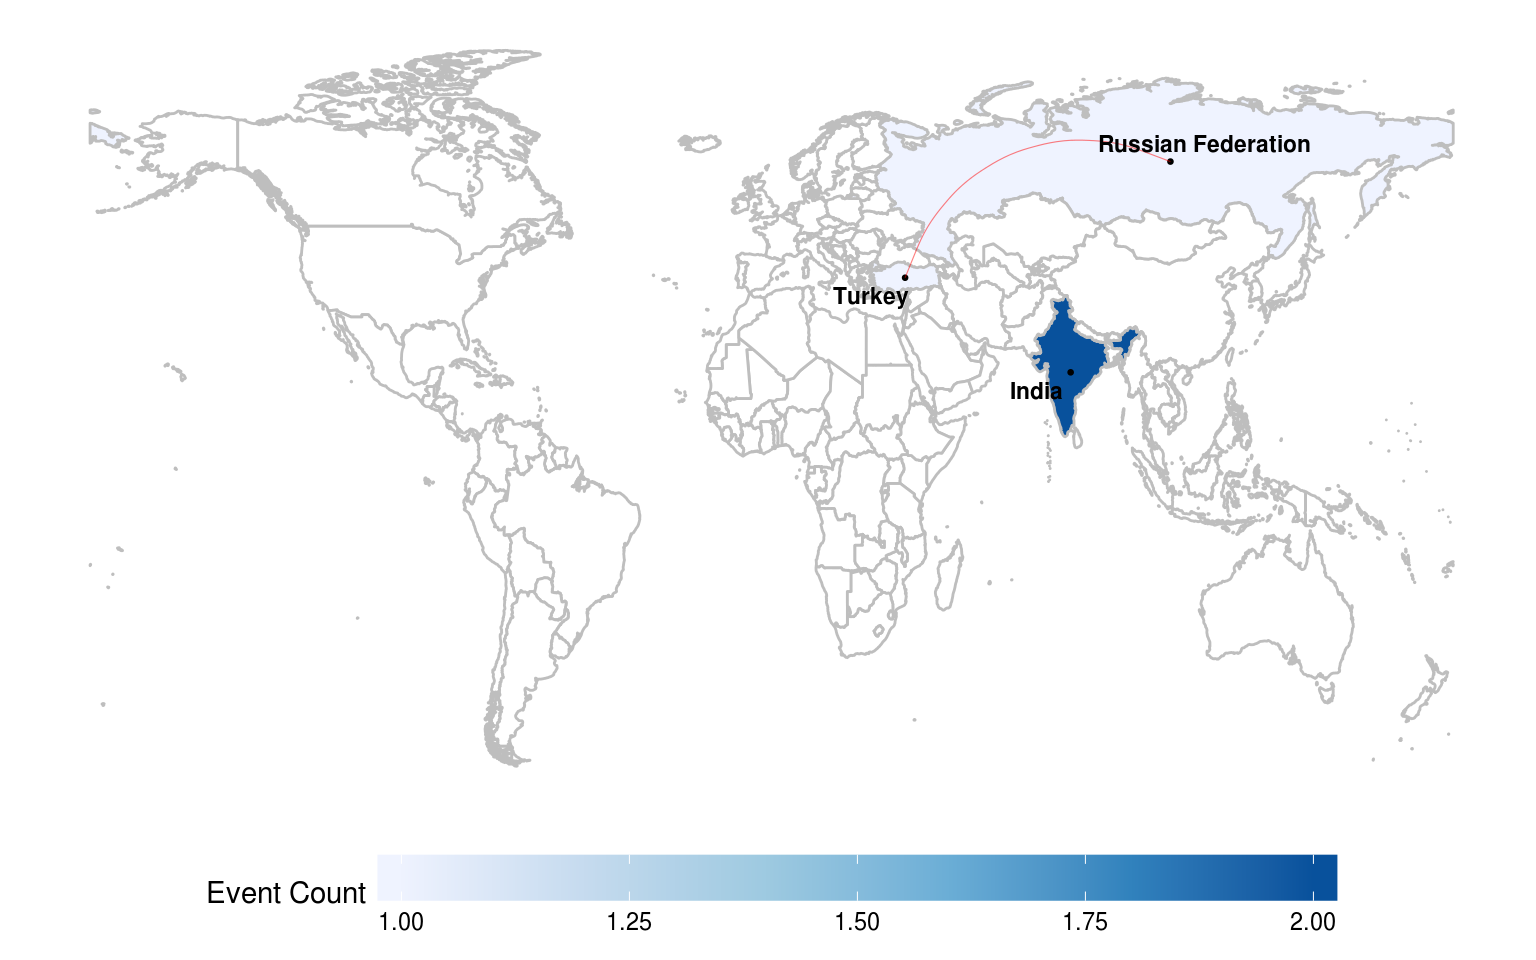
\includegraphics{_main_files/figure-latex/unnamed-chunk-10-1.pdf}

\subsection{Most Active in Last 7
Days}\label{most-active-in-last-7-days}

\begin{Shaded}
\begin{Highlighting}[]
\NormalTok{event_summary <-}\StringTok{ }\KeywordTok{get_event_summary}\NormalTok{(events, country_centroids, }\DataTypeTok{period =} \DecValTok{7}\NormalTok{)}
\KeywordTok{show_top10}\NormalTok{(}\KeywordTok{select}\NormalTok{(event_summary$nodes, CountryName, EventCount))}
\end{Highlighting}
\end{Shaded}

\begin{tabular}{l|r}
\hline
CountryName & EventCount\\
\hline
United States & 525\\
\hline
Russian Federation & 113\\
\hline
United Kingdom & 81\\
\hline
Israel & 77\\
\hline
Germany & 76\\
\hline
India & 57\\
\hline
Iran, Islamic Republic of & 51\\
\hline
Turkey & 42\\
\hline
Mexico & 37\\
\hline
Ukraine & 33\\
\hline
\end{tabular}

\begin{Shaded}
\begin{Highlighting}[]
\KeywordTok{show_top10}\NormalTok{(}\KeywordTok{select}\NormalTok{(event_summary$edges, CountryA, CountryB, EventCount))}
\end{Highlighting}
\end{Shaded}

\begin{tabular}{l|l|r}
\hline
CountryA & CountryB & EventCount\\
\hline
Iran, Islamic Republic of & United States & 43\\
\hline
United Kingdom & United States & 35\\
\hline
Germany & Turkey & 34\\
\hline
Israel & United States & 34\\
\hline
Russian Federation & United States & 33\\
\hline
Korea, Republic of & United States & 24\\
\hline
Australia & United States & 22\\
\hline
India & United States & 20\\
\hline
Mexico & United States & 19\\
\hline
United Kingdom & Israel & 17\\
\hline
\end{tabular}

\begin{Shaded}
\begin{Highlighting}[]
\KeywordTok{plot_activity}\NormalTok{(world_map, event_summary)}
\end{Highlighting}
\end{Shaded}

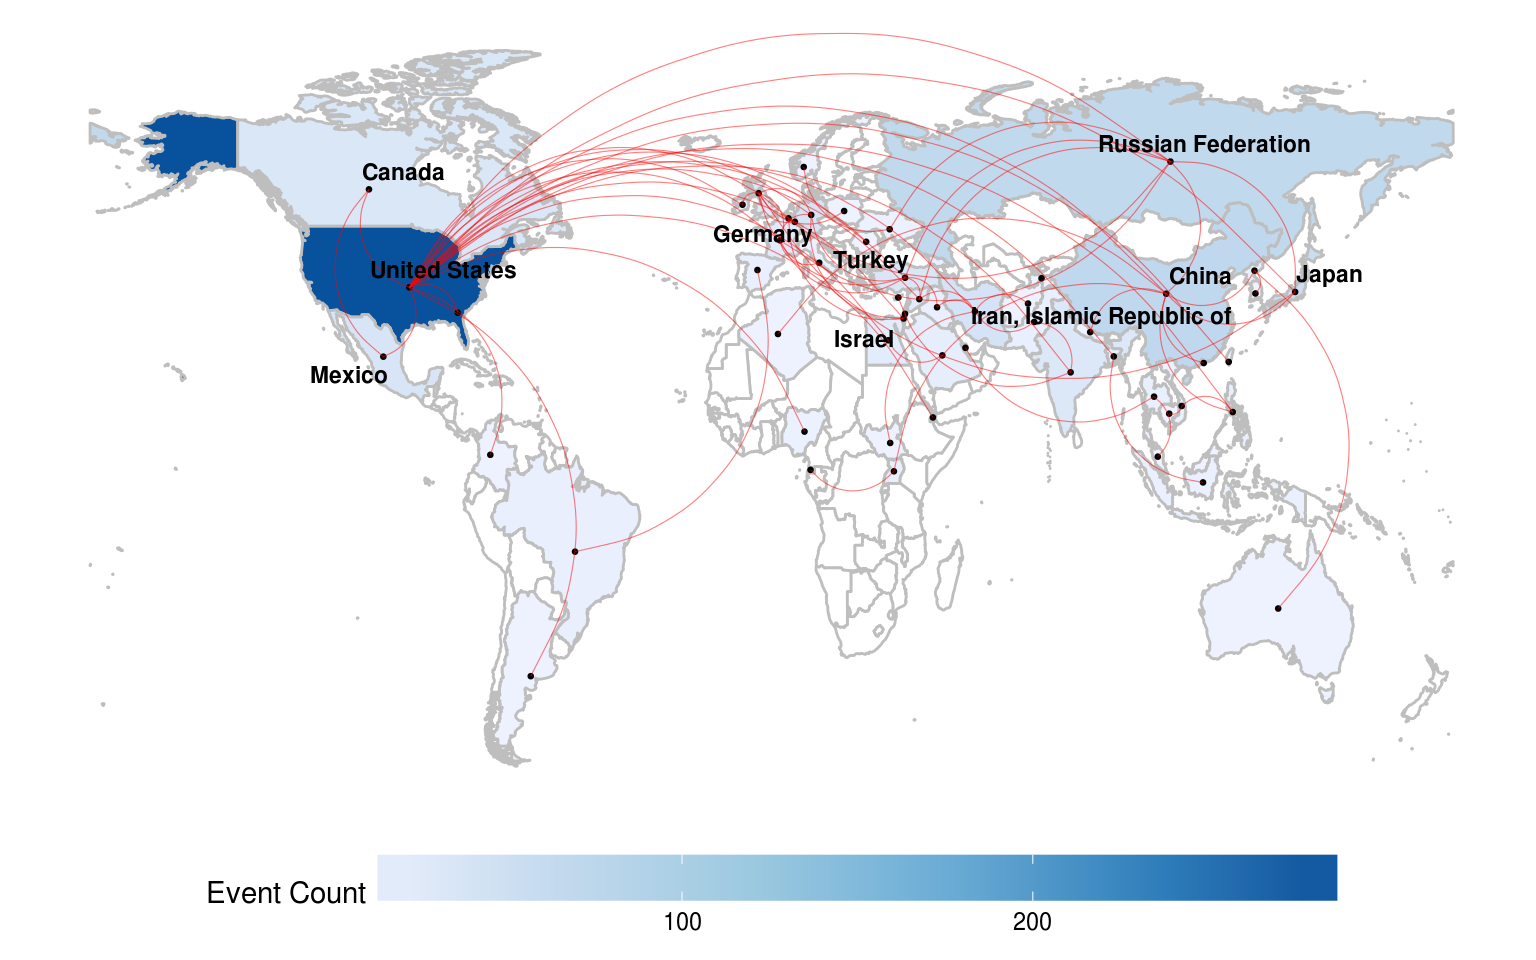
\includegraphics{_main_files/figure-latex/unnamed-chunk-11-1.pdf}

\subsection{Most Active in Last 30
Days}\label{most-active-in-last-30-days}

\begin{Shaded}
\begin{Highlighting}[]
\NormalTok{event_summary <-}\StringTok{ }\KeywordTok{get_event_summary}\NormalTok{(events, country_centroids, }\DataTypeTok{period =} \DecValTok{30}\NormalTok{)}
\KeywordTok{show_top10}\NormalTok{(}\KeywordTok{select}\NormalTok{(event_summary$nodes, CountryName, EventCount))}
\end{Highlighting}
\end{Shaded}

\begin{tabular}{l|r}
\hline
CountryName & EventCount\\
\hline
United States & 2167\\
\hline
United Kingdom & 407\\
\hline
Russian Federation & 404\\
\hline
Israel & 243\\
\hline
Germany & 236\\
\hline
Iran, Islamic Republic of & 197\\
\hline
China & 186\\
\hline
India & 177\\
\hline
Mexico & 161\\
\hline
Turkey & 143\\
\hline
\end{tabular}

\begin{Shaded}
\begin{Highlighting}[]
\KeywordTok{show_top10}\NormalTok{(}\KeywordTok{select}\NormalTok{(event_summary$edges, CountryA, CountryB, EventCount))}
\end{Highlighting}
\end{Shaded}

\begin{tabular}{l|l|r}
\hline
CountryA & CountryB & EventCount\\
\hline
Russian Federation & United States & 224\\
\hline
United Kingdom & United States & 188\\
\hline
Israel & United States & 152\\
\hline
Mexico & United States & 111\\
\hline
Iran, Islamic Republic of & United States & 109\\
\hline
India & United States & 78\\
\hline
Germany & United States & 54\\
\hline
Germany & France & 44\\
\hline
Germany & Turkey & 41\\
\hline
United Kingdom & Turkey & 40\\
\hline
\end{tabular}

\begin{Shaded}
\begin{Highlighting}[]
\KeywordTok{plot_activity}\NormalTok{(world_map, event_summary)}
\end{Highlighting}
\end{Shaded}

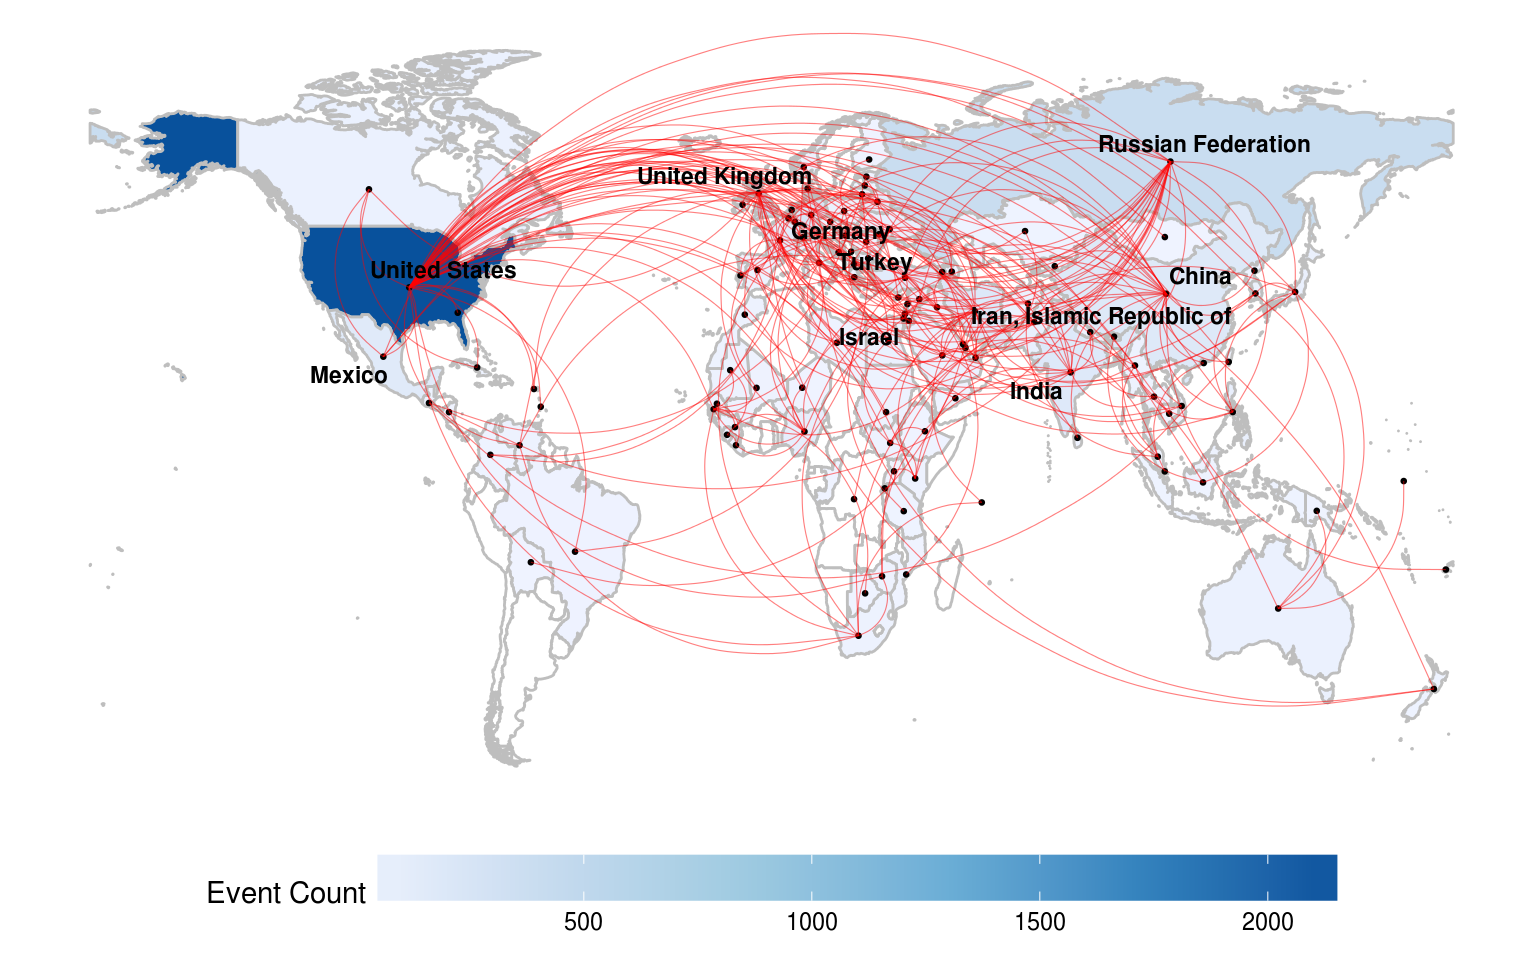
\includegraphics{_main_files/figure-latex/unnamed-chunk-12-1.pdf}

\end{document}
